\newpage
\section{System}
\subsection{System Architecture}

We have implemented \system\ as a web-based tool on top of a PostgreSQL database. In Figure X we present the system architecture of \system\ , which consists of three core modules: the traversal module, the query module, and the stats module. The traversal module contains several alternative algorithms for traversing the visualization hierarchy. These algorithms are responsible for both generating the visualization hierarchy and identifying the solution (dashboard) from the hierarchy. For generating the visualization hierarchy, the traversal module passes the list of visualizations to be generated to the query module. The query module translates these visualizations into queries, and then optimizes (by grouping) and executes the queries. The stats module is an optional module that allows the traversal module to prune low-utility visualizations without actually generating them. Specifically, it generates coarse statistics for the unexplored visualizations based on the current list of explored visualizations. 

\begin{center}
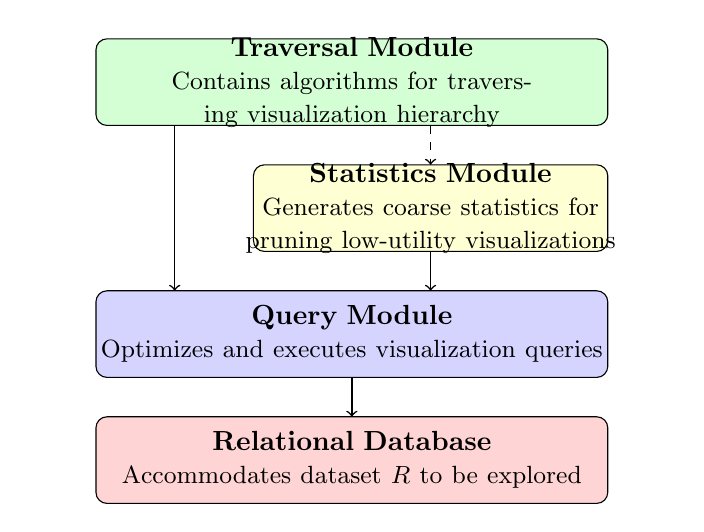
\begin{tikzpicture}
    \filldraw [fill={rgb:red,1;white,5}, rounded corners=4pt] (0, 0) rectangle (6.5, 1.1) node[pos=.5, align=center, text width=8cm] {\textbf{Relational Database}\\ {\small Accommodates dataset $R$ to be explored}};
    \filldraw [fill={rgb:blue,1;white,5}, rounded corners=4pt] (0, 1.6) rectangle (6.5, 2.7) node[pos=.5, align=center, text width=8cm] {\textbf{Query Module}\\ {\small Optimizes and executes visualization queries}};
    \filldraw [fill={rgb:yellow,1;white,5}, rounded corners=4pt] (2, 3.2) rectangle (6.5, 4.3) node[pos=.5, align=center, text width=5cm] {\textbf{Statistics Module}\\ {\small Generates coarse statistics for pruning low-utility visualizations}};
    \filldraw [fill={rgb:green,1;white,5}, rounded corners=4pt] (0, 4.8) rectangle (6.5, 5.9) node[pos=.5, align=center, text width=8cm] {\textbf{Traversal Module}\\ {\small Contains algorithms for traversing visualization hierarchy}};
    \draw [->, line width=0.2mm] (1, 4.8) -- (1, 2.7);
    \draw [->, dashed, line width=0.2mm] (4.25, 4.8) -- (4.25, 4.3);
    \draw [->, line width=0.2mm] (4.25, 3.2) -- (4.25, 2.7);
    \draw [->, line width=0.2mm] (3.25, 1.6) -- (3.25, 1.1);
\end{tikzpicture}
\end{center}

\subsection{Algorithms}
We give an overview of the traversal algorithms to generate the visualization hierarchy and identify visualizations from this hierarchy. We start with offline approach where we first generate the complete hierarchy of visualizations, and then work towards identifying the maximum utility solution. Then, we present our online algorithms to identify a solution in a single phase. 


\subsection{User Interaction}

\subsection{Assistive tools for visualizing large lattices}
Due to the amount of space occupied by the hierarchical layout when the numbers of visualizations gets large, we have developed tools to help users navigate through difference parts of the dashboard interactively. 
\textbf{Navigation Tools:} As shown in Figure ---, the system provides toolbar buttons with keyboard binding to zoom in, out, and extent as well as moving around the canvas. Alternatively, participants can also zoom and pan with mouse click and scroll.  

minimap and

collapsing redundant sibling visualizations
